\subsection{Subsystem 3: Text Display \& Chassis}
% Subsystem Diagram
\subsubsection{Subsystem Diagrams}
\begin{figure}[h]
    \centering
    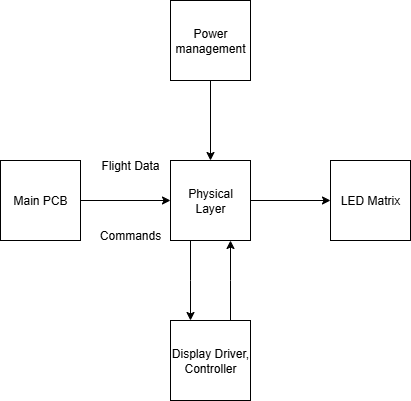
\includegraphics[width=12cm]{images/DisplayDriver/blockDiagram-display.png} % Change the picture
    \caption{Display subsystem Block Diagram}
\end{figure} % If your subsystem is more coding, change it to activity diagram

% Specifications
\subsubsection{Specifications}
\begin{enumerate}
    \item Feature a 2056-pixel Dot Display (128 x 256px)
    \item Physical dimensions of housing within 5\% of 64 x 128 x 256 mm.
\end{enumerate}

% Subsystem Interactions
\subsubsection{Subsystem Interactions}
The display subsystem links the main PCB and the LED Matrix. This subsystem will interface with the power management system and the main PCB. It will recieve data and commands from the main PCB, interpret the commands, and display the data.

% Core ECE
\subsubsection{Core ECE Design Tasks}
\begin{itemize}
    \item \textbf{ECE 27000}: Provides a solid foundation in logic circuits. Helps for designing registers, data paths, logic that drives the LED panel.
    \item \textbf{ECE 25500}: Provides a base understanding of transisters, amplifiers, and fundamentals into I-V behavior.
    \item \textbf{ECE 40862}: Teaches valuable STM concepts such as programming, interrupts, and DMA which are needed to drive the display controller efficiently.
\end{itemize}

% Schematics
\subsubsection{Schematics}

\begin{figure}[H]
    \centering
    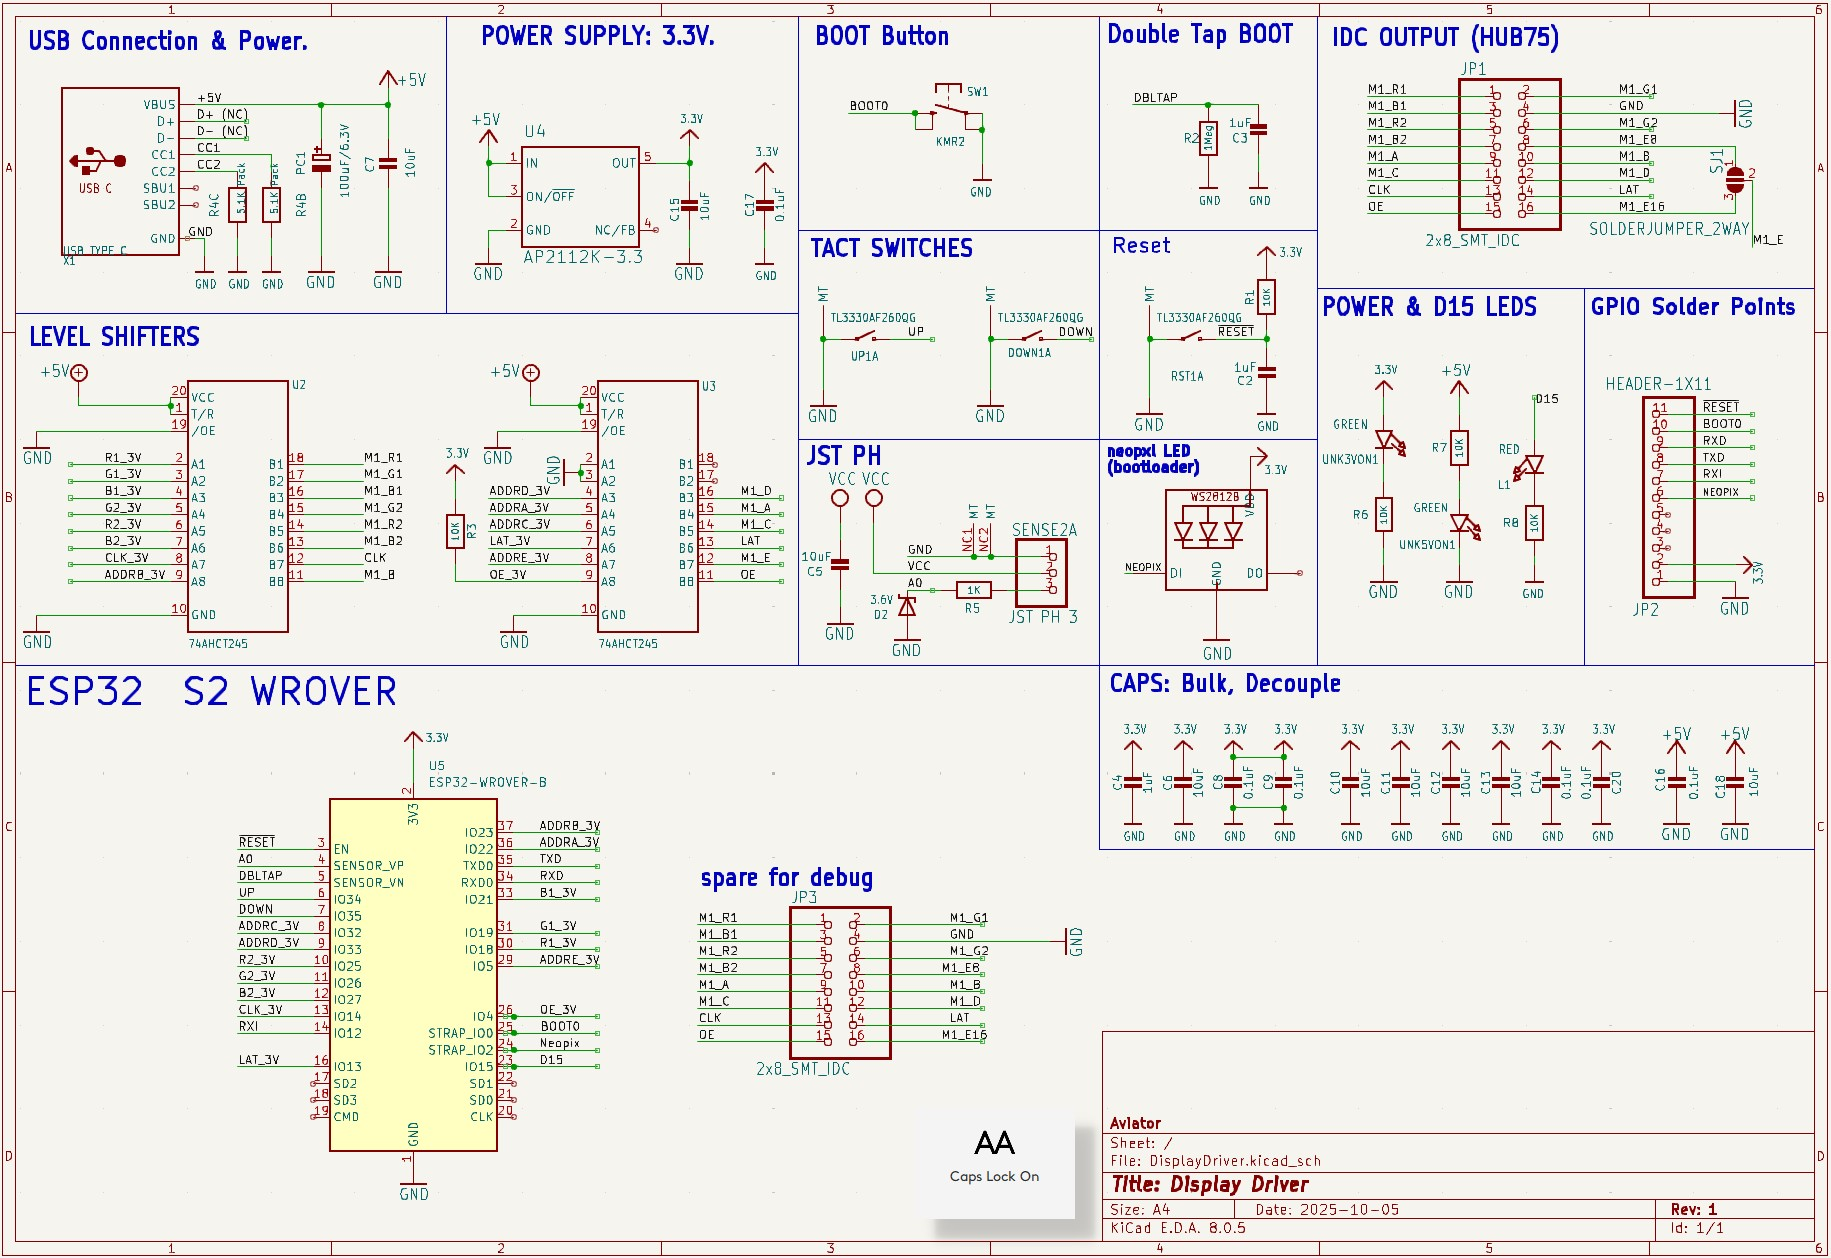
\includegraphics[width=12cm]{images/DisplayDriver/DisplayDriver Schematic.jpg}
    \caption{Display Driver Schematic}
\end{figure}

\begin{figure}[H]
    \centering
    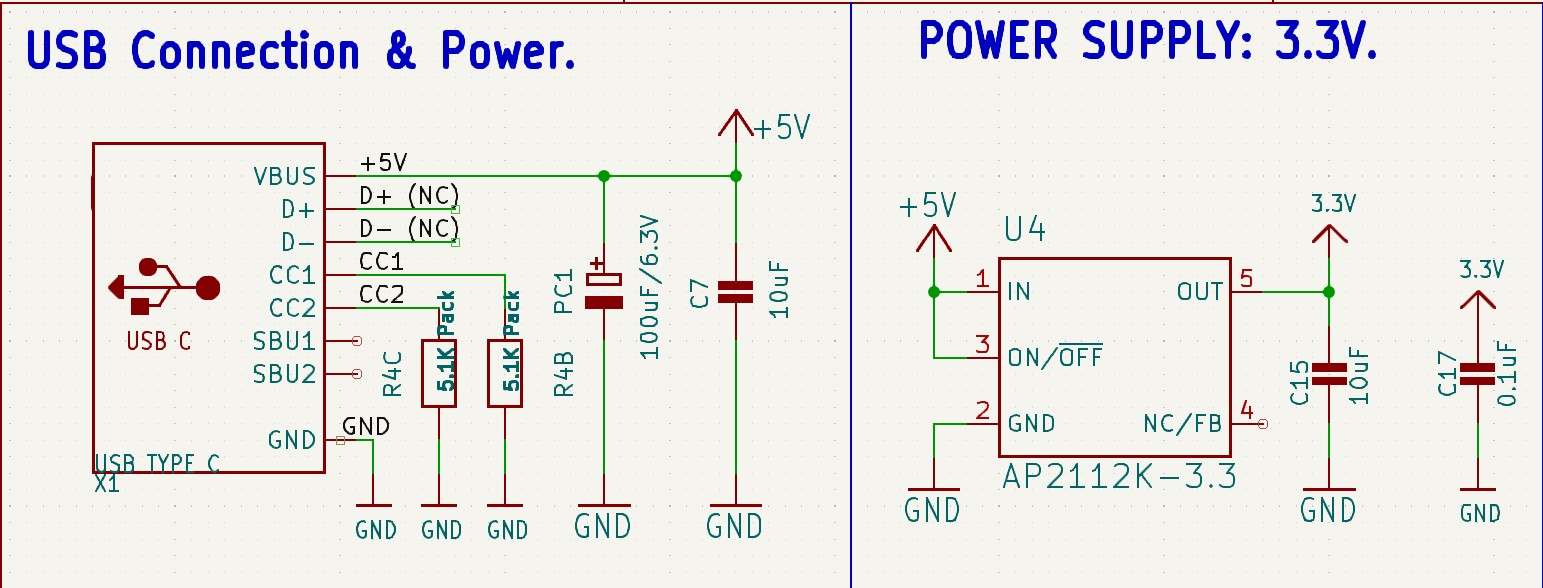
\includegraphics[width=12cm]{images/DisplayDriver/USBPwrGeneric.jpg}
    \caption{Generic temp power input}
\end{figure}

\begin{figure}[H]
    \centering
    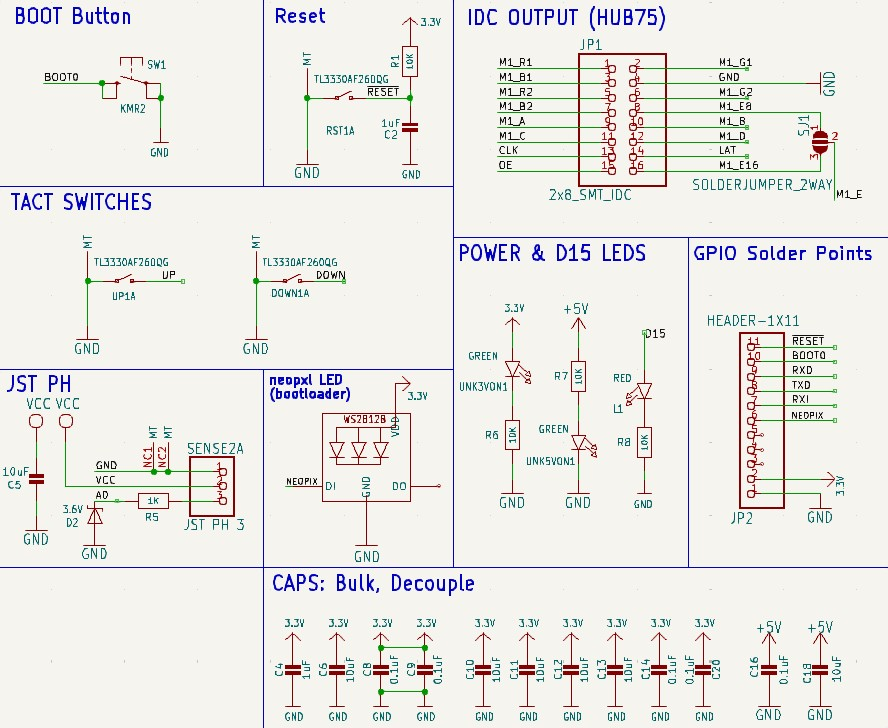
\includegraphics[width=12cm]{images/DisplayDriver/DriverBoardFeatures.jpg}
    \caption{Features of Display Driver Board}
\end{figure}

\begin{figure}[H]
    \centering
    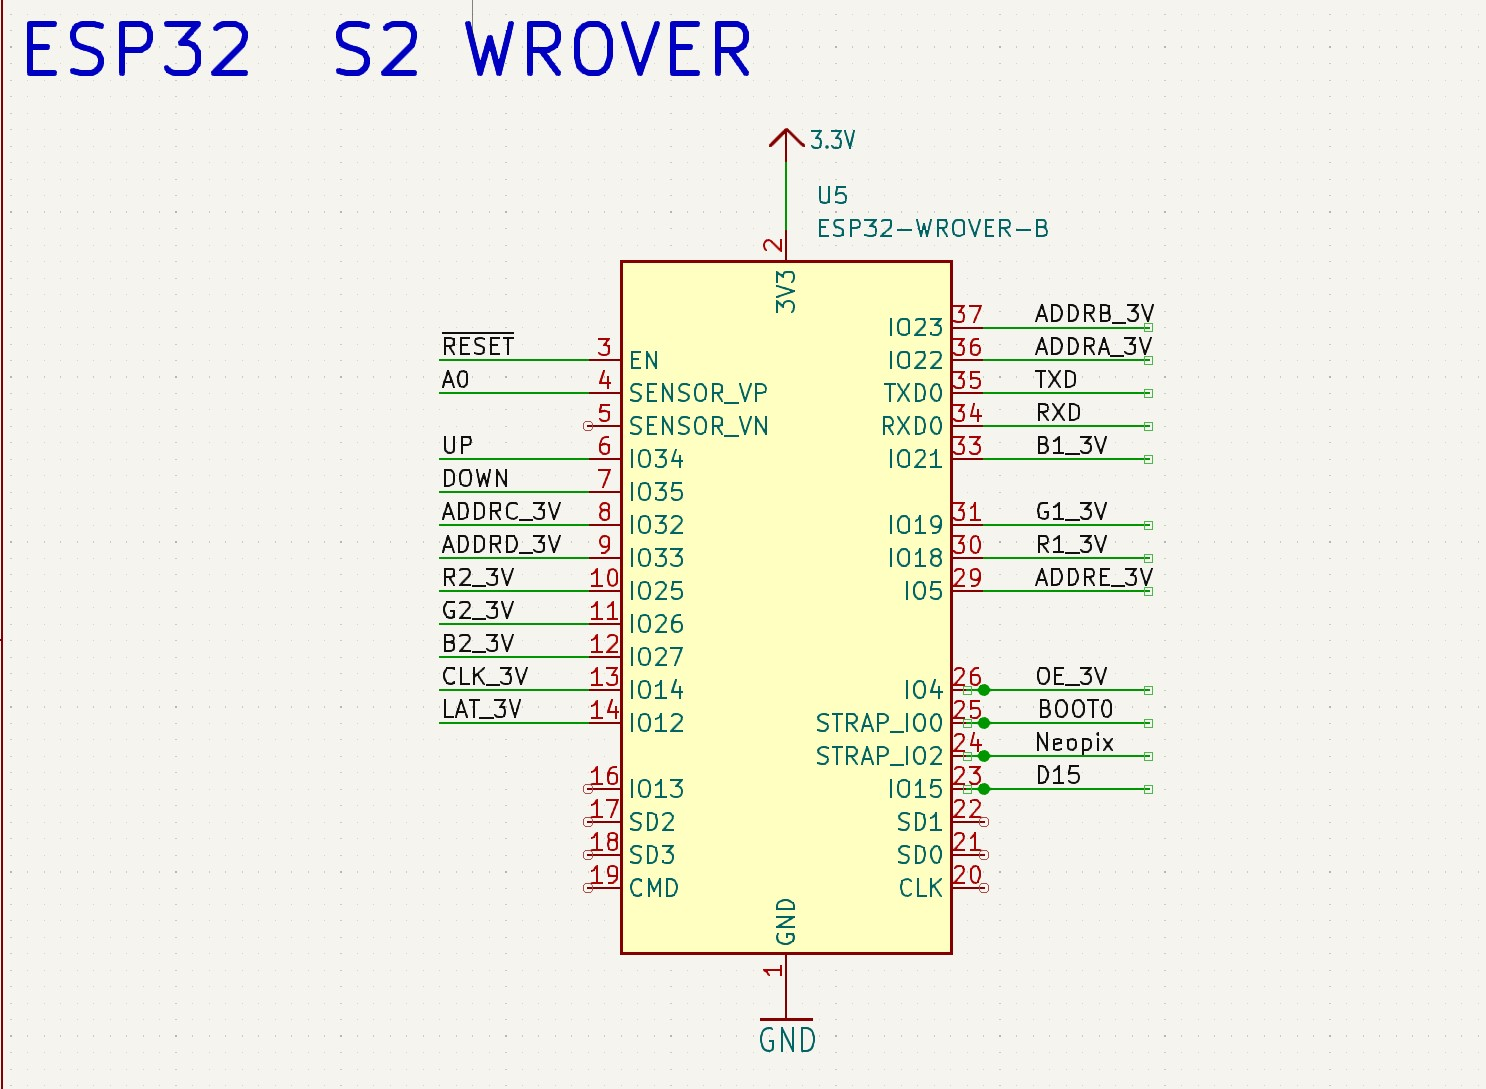
\includegraphics[width=12cm]{images/DisplayDriver/WroverUsage.jpg}
    \caption{Pinout of the ESP32-S2 WROVER-B}
\end{figure}

\FloatBarrier

% Parts List
\subsubsection{Parts}
\begin{itemize}
    \item 32 x 64 px LED Matrix (ADAFruit from DigiKey)
    \item Custom PCB (possibly a hat or extension) for driving display
\end{itemize}

\subsection{Finalized Parts}
\begin{itemize}
    \item 74AHCT244 (2)
    \item WS2812B (1)
    \item PCB Headers:
    \begin{itemize}
        \item JST PH 3 (1)
        \item 2x08 SMT IDC (2)
    \end{itemize}
    \item Resistors:
    \begin{itemize}
        \item see schematic. / w.i.p.
    \end{itemize}
    \item Capacitors
    \begin{itemize}
        \item see schematic. / w.i.p.
    \end{itemize}
    \item Diodes 
    \begin{itemize}
        \item see schematic. / w.i.p.
    \end{itemize}
    \item Switches and Buttons
    \begin{itemize}
        \item see schematic. / w.i.p.
    \end{itemize}
\end{itemize}
% Algorithm
\subsubsection{Algorithm}

\begin{lstlisting}
    Initialize:
    Configure GPIOs (DATA, CLK, LAT, OE, row select lines (A,B,C,D))
    Initialize interface for incoming data
    Initialize timer for refresh interrupts
    Set PWM resolution (e.g., 8-bit)

    Main Loop:
    while (true):
        if new frame data available from main PCB:
            copy frame buffer into local memory (double buffer optional)
        
        for each row_index in 0 .. NUM_ROWS-1:
            select_row(row_index)        
            OE = HIGH                   
            
            for pwm_bit = 7 downto 0:    // for 8-bit PWM
                for col_index = 0 .. NUM_COLS-1:
                    pixel = frame_buffer[row_index][col_index]
                    if pixel.red  & (1 << pwm_bit) != 0:
                        DATA_R = HIGH
                    else:
                        DATA_R = LOW
                    if pixel.green & (1 << pwm_bit) != 0:
                        DATA_G = HIGH
                    else:
                        DATA_G = LOW
                    if pixel.blue & (1 << pwm_bit) != 0:
                        DATA_B = HIGH
                    else:
                        DATA_B = LOW
                    
                    pulse(CLK)           
                    
                pulse(LAT)                
                OE = LOW                   
                delay(PWM_DELAY[pwm_bit])  
                
        repeat indefinitely
\end{lstlisting}

% Theory of Operation
\subsubsection{Theory of Operation}
The Display Driver subsystem serves as the primary interface between the ESP32-WROVER-B microcontroller and a 32×64 HUB75 RGB LED matrix, enabling real-time visualization of aviation and weather data. 
The ESP32 handles pixel generation, frame buffering, and timing control for row and column scanning of the display. 
Core signals — including LAT (latch), OE (output enable), CLK (clock), and address lines A–E — are driven directly from the ESP32’s GPIO pins and level-shifted from 3.3 V logic to the 5 V domain required by the HUB75 interface. 
The RGB data lines (R1, G1, B1, R2, G2, B2) are similarly translated to ensure proper color channel switching for both the upper and lower halves of the LED matrix. 
During operation, the ESP32 continuously cycles through the address lines, updating one row at a time while controlling brightness through pulse-width modulation synchronized with the OE signal. 
Power is supplied through regulated 5 V and 3.3 V rails, supporting both the LED panel and logic circuitry. 
Optional pushbuttons provide manual reset and boot functionality, while status LEDs indicate system power and data activity. 
In system deployment, the Display Driver operates under firmware that retrieves aircraft position and weather telemetry from networked sources, translating this incoming data into color-coded graphical output. 
This modular design allows the subsystem to function independently or as an integrated component of the larger Aviator platform, emphasizing robustness, timing precision, and electrical isolation between logic and display domains.

% Specification Measurement
\subsubsection{Specifications Measurement}
[\textbf{DD3+} Every specification here should match the specification above. ]
\begin{enumerate}
    \item {[Copy specification here. ]} \\
          {[Explain the specification here. Add photoes if necessary. ]}
\end{enumerate}

% Standards
\subsubsection{Standards}
\begin{itemize}
    \item \textbf{IEC 61010}: Safety for low-voltage electronic equipment; ensures protection against shorts, overcurrent, and handling risks.
    \item \textbf{SPI/I²C}: If MCU/controller communicates with peripheral ICs over standard buses.
    \item \textbf{HUB75}: Standard for 32×64 RGB LED matrices; timing, row multiplexing, and data latching must be followed.
    \item \textbf{JESD51}: Important for high-current LED arrays; ensures heat dissipation and junction temperatures are within safe limits.
\end{itemize}